\section{Conjugate sets}
\subsection{Problem №1}
Find the sets $\mathds{S}^*, \mathds{S}^{**}, \mathds{S}^{***}$, if

\begin{equation*}
    \mathds{S} = \{ x \in \mathds{R}^2 \text{ | } x_1 + x_2 \geq -1, \text{ } 2x_1 - x_2 \geq 0, \text{ } -x_1+2x_2\leq -2\}
\end{equation*}

\underline{\textbf{Solution:}}
S is closed, convex and includes 0, then $S^{**} = S$, $S^{***} = S^{*}$. 

\begin{equation*}
    S = conv \left\{ 
        \begin{pmatrix} 0  \\ -1 \end{pmatrix}, 
        \begin{pmatrix} \frac{-1}{3} \\ \frac{-2}{3} \end{pmatrix} \right\} 
    + cone \left\{ 
        \begin{pmatrix} 2  \\ 1  \end{pmatrix}, 
    \begin{pmatrix} 1  \\ 2  \end{pmatrix} \right\}
\end{equation*}

\begin{center}
\fbox{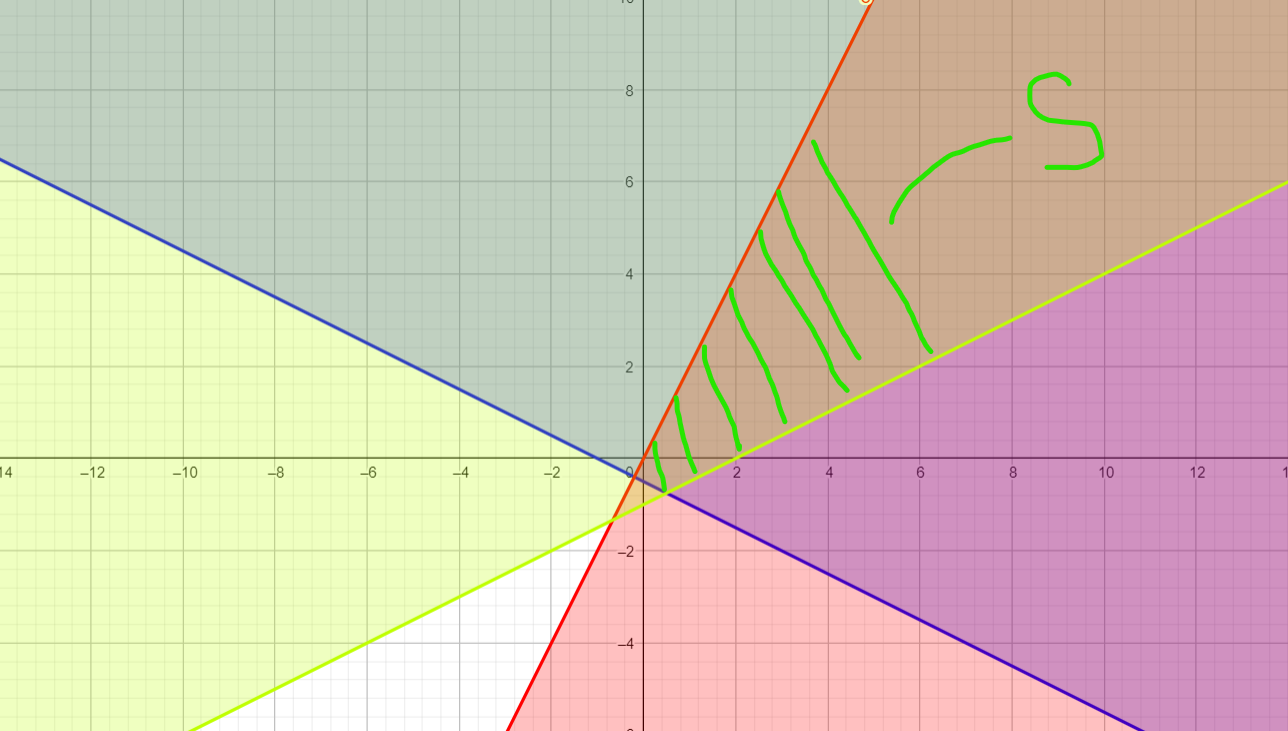
\includegraphics[width=\textwidth]{pictures/task_05_01.png}}
\end{center}

And then we get this:
\begin{equation*}
    \begin{cases}
    0\cdot p_1 - p_2 \geq -1 \\
    -\frac{1}{3} p_1 - \frac{2}{3}p_2 \geq -1 \\
    2 p_1 + p_2 \geq 0 \\
    p_1 + 2p_2 \geq 0
    \end{cases}
\end{equation*}

\begin{equation*}
    \begin{cases}
    p_2 \leq 1 \\
    p_1 + 2p_2 \leq 3 \\
    2 p_1 + p_2 \geq 0 \\
    p_1 + 2p_2 \geq 0
    \end{cases}
\end{equation*}


And we get:
\begin{equation*}
    S^{*} = conv \left\{ 
        \begin{pmatrix} \frac{-1}{2}  \\ 1 \end{pmatrix}, 
        \begin{pmatrix} 1 \\ 1 \end{pmatrix},
        \begin{pmatrix} 0 \\ 0 \end{pmatrix} \right\} 
        + cone \left\{ 
        \begin{pmatrix} 2  \\ -1  \end{pmatrix} \right\}
\end{equation*}

\begin{center}
   \fbox{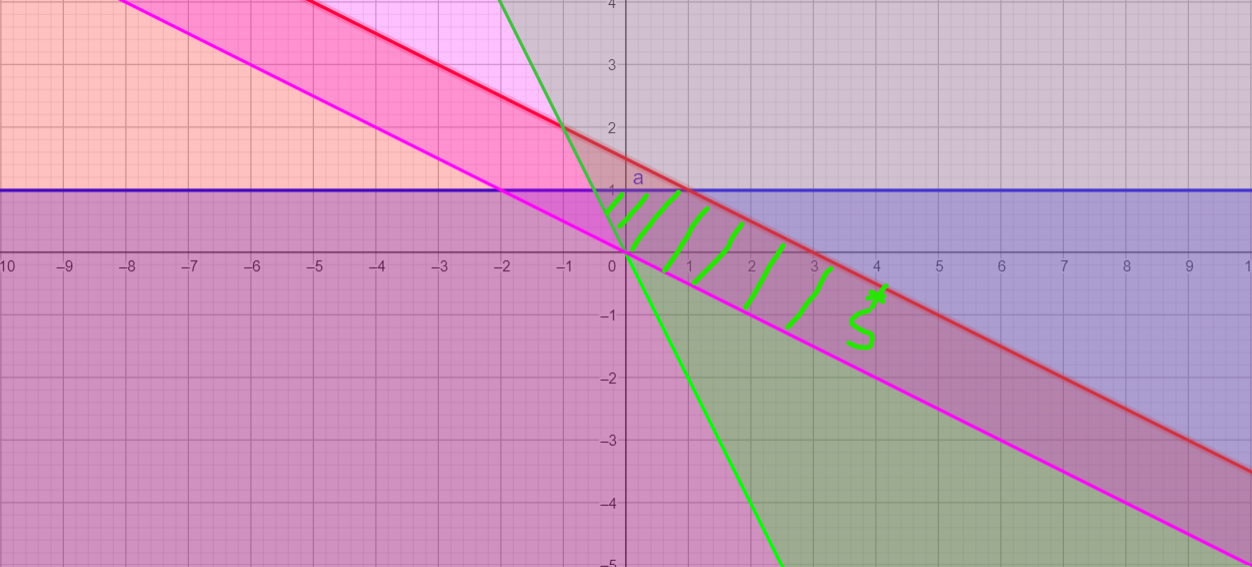
\includegraphics[width=\textwidth]{pictures/task_05_02.png}}
\end{center}

\begin{equation*}
    \begin{cases}
        -\frac{1}{2}p_1 + p_2 \geq -1 \\
        p_1 + p_2 \geq -1 \\
        2p_1 - p_2 \geq 0
    \end{cases}
\end{equation*}

\begin{equation*}
    S^{**} = conv \left\{ 
        \begin{pmatrix} 0  \\ -1 \end{pmatrix}, 
        \begin{pmatrix} \frac{-1}{3} \\ \frac{-2}{3} \end{pmatrix} \right\} 
    + cone \left\{ 
        \begin{pmatrix} 2  \\ 1  \end{pmatrix}, 
    \begin{pmatrix} 1  \\ 2  \end{pmatrix} \right\}
\end{equation*}

\begin{center}
    \fbox{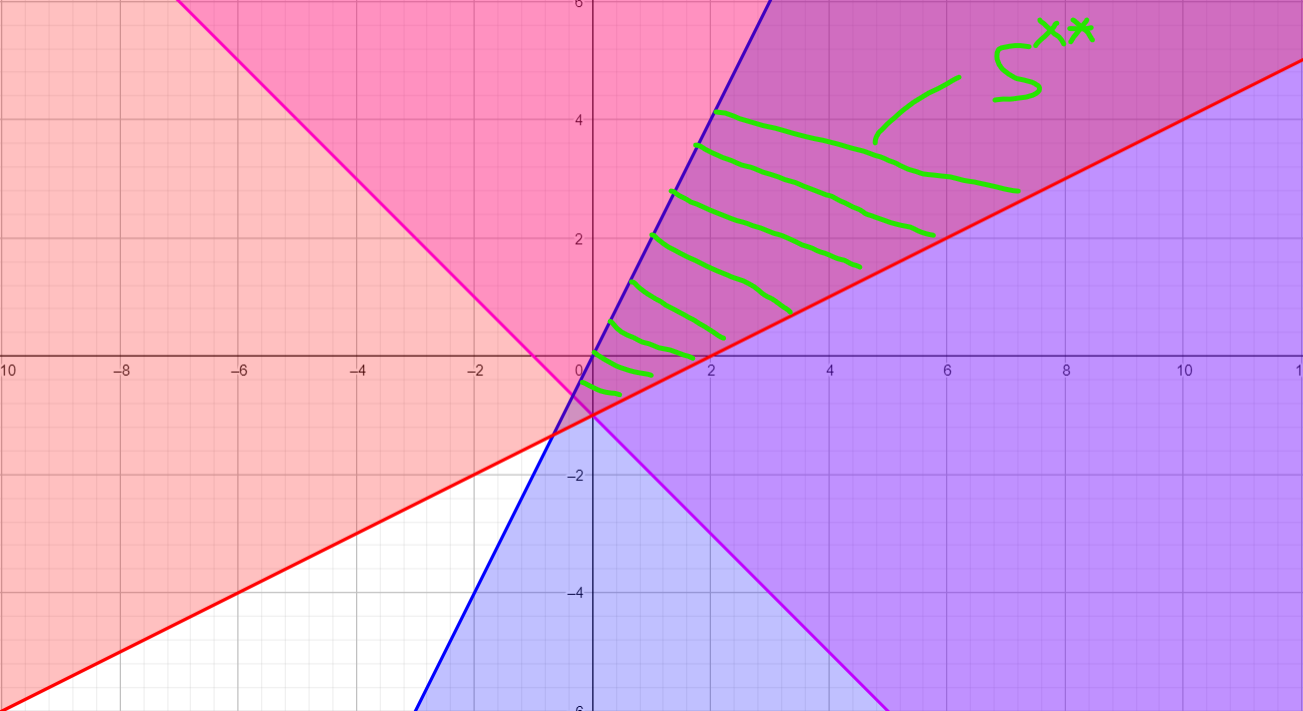
\includegraphics[width=\textwidth]{pictures/task_05_03.png}}
\end{center}

$S^{***}$ the same as $S^{*}$. I draw $S^{**}$ to demonsrate that they are similar.

\underline{\textbf{Answer:}} All answers are above.

\subsection{Problem №2}
Prove, that $K_p$ and $K_{p^*}$ are inter-conjugate, i.e. $(K_p)^* = K_{p^*}$, $(K_{p^*})^* = K_p$, where $K_p = \left\{ [x, \mu] \in \mathds{R}^{n+1} : ||x||_p \leq \mu \right\}$, $1 < p < \infty$ is the norm cone (w.r.t p - norm) and $p, p_{*}$ are conjugated, i.e. $p^{-1} + p_{*}^{-1} = 1$. You can assume, that $p_* = \infty$ if $p = 1$ and viceversa.

\underline{\textbf{Solution:}}
$K := \{ x \in \mathds{R}^n \text{ } | \text{ } ||x|| \leq 1 \} $
Unit ball is convex, symmetric by x and closed, norm we can write in such way: $||x|| = \frac{1}{\sup \{t \geq 0 \text{ } | \text{ } tx \in K \} }$.

From properties of conjugate norm: $(||x||_p)^* = ||x||_{p^*}$, if $p^{-1} + p_*^{-1} = 1$.

We have finite-dimensional space, then will be executed $||x||_{**} = ||x||, \forall x$

Wohoo, we proved.

\subsection{Problem №3}
The cone $\mathds{R}_{+}^n$ fits for it. $x^Ty \geq 0$ $\forall x \succcurlyeq 0$ $\Longleftrightarrow$ $y \succcurlyeq 0$ and it's $\mathds{R}_{+}^n$.

\subsection{Problem №4}
Find the conjugate set to the ellipsoid:
\begin{equation*}
    S = \left\{ x \in \mathds{R}^n | \sum\limits_{i=1}^n a_i^2x_i^2 \leq \varepsilon^2 \right\}
\end{equation*}

\underline{\textbf{Solution:}}
It's equivalent to:
\begin{equation*}
    S = \left\{ x \in \mathds{R}^n | \sum\limits_{i=1}^n a_i^2x_i^2 \leq \varepsilon^2 \right\}
\end{equation*}
$A = diag(\frac{a_i}{\varepsilon})$
\begin{equation*}
    ||Ax||_2^2 = \sum\limits_{i=1}^n (\frac{a_i}{\varepsilon})^2x_i^2
\end{equation*}

From Boyd's optimization I know that:
\begin{equation*}
S = \{ x \in \mathds{R}^n \text{ } | \text{ }||Ax||_2 \leq 1 \} = E = \{ A^{-1}u \text{ } | \text{ } ||u||_2 \leq 1\}    
\end{equation*}
$A^{-1} = diag(\frac{\epsilon}{a_i})$. 

Let's show that it's true.
\newline
1. $E \subseteq S$: $x = A^{-1}u$, $||u||_2 \leq 1$ in S: $||AA^{-1}u||_2 \leq 1$, therefore $E \subseteq S$ it's true.
\newline
2. $S \subseteq E$: $||Ax||_2 \leq 1$, $z = Ax$, $||z||_2 \leq 1$, $x = A^{-1}z$, $||z||_2 \leq 1$, therefore $x\ \in E$, $\hookrightarrow S \subseteq E$

We prove that it's true. 

We need find all $p \in E^* : \forall x \in E$, $\langle p, x \rangle \geq -1$, $\forall x = A^{-1}u$, $||u||_2 \leq 1$, 
\begin{equation*}
\langle p, A^{-1}u \rangle = \langle A^{-T}p, u \rangle \geq -1    
\end{equation*}

From cauchy-bunyakovsky and $||u||_2 \leq 1$ we get:
\begin{equation*}
    |\langle A^{-T}p, u \rangle|\leq ||u||_2 \cdot ||A^{-T}p||_2 \leq ||A^{-T}p||_2 
\end{equation*}

We are suitable for all p, for which is true: $\langle A^{-T}p, u \rangle = - ||A^{-T}p||_2$,
$-||A^{-T}p||_2 \geq -1$, we get:
\begin{equation*}
    ||A^{-T}p||_2 \leq 1
\end{equation*}
This sets an ellips with matrix $A^{-T} = diag(\frac{\varepsilon}{a_i})$.

\begin{equation*}
    S^* = E^* = \left\{ x \in \mathds{R}^n | \sum\limits_{i=1}^n (\frac{\varepsilon}{a_i})^2 x_i^2 \leq 1 \right\}
\end{equation*}

\underline{\textbf{Answer:}}

\begin{equation*}
    S^* = \left\{ x \in \mathds{R}^n | \sum\limits_{i=1}^n (\frac{1}{a_i})^2 x_i^2 \leq \frac{1}{\varepsilon^2} \right\}
\end{equation*}


\subsection{Problem №5}
Find the conjugate cone for the exponential cone:
\begin{equation*}
    K = \left\{ (x, y, z) | y > 0\text{, } ye^{\frac{x}{y}} \leq z \right\}
\end{equation*}

\underline{\textbf{Solution:}}
By definition of conjugate set: 

\begin{equation*}
\begin{cases}
    a x + b y + c z \geq 0 \\
    y > 0 \\
    y e^{\frac{x}{y}} \leq z
\end{cases}, \text{let's take: $t = \frac{x}{y}, p = \frac{z}{y}$, }
\begin{cases}
    at + b + cp \geq 0 \\
    p \geq e^t \\
    p \leq 0
\end{cases}
\end{equation*}
\begin{enumerate}
    \item $c = 1$, let's take a and b in such way that all values lie above $p \geq e^t$.
    \begin{enumerate}
        \item $a > 0$: $\not \exists b$
        \item $a = 0$: $b \geq 0$
        \item $a < 0$: $\begin{cases}
            p \geq e^t \\
            p \geq - b - at
        \end{cases}$, $\begin{cases} 
        p' = e^t \\ 
        p' = -a  \\
        \end{cases}$, $\begin{cases}
            t = \ln(-a) \\
            p = -a 
        \end{cases}$, 
        $b \geq a(1-\ln(-a))$
    \end{enumerate}


\begin{figure}
  \centering
    \fbox{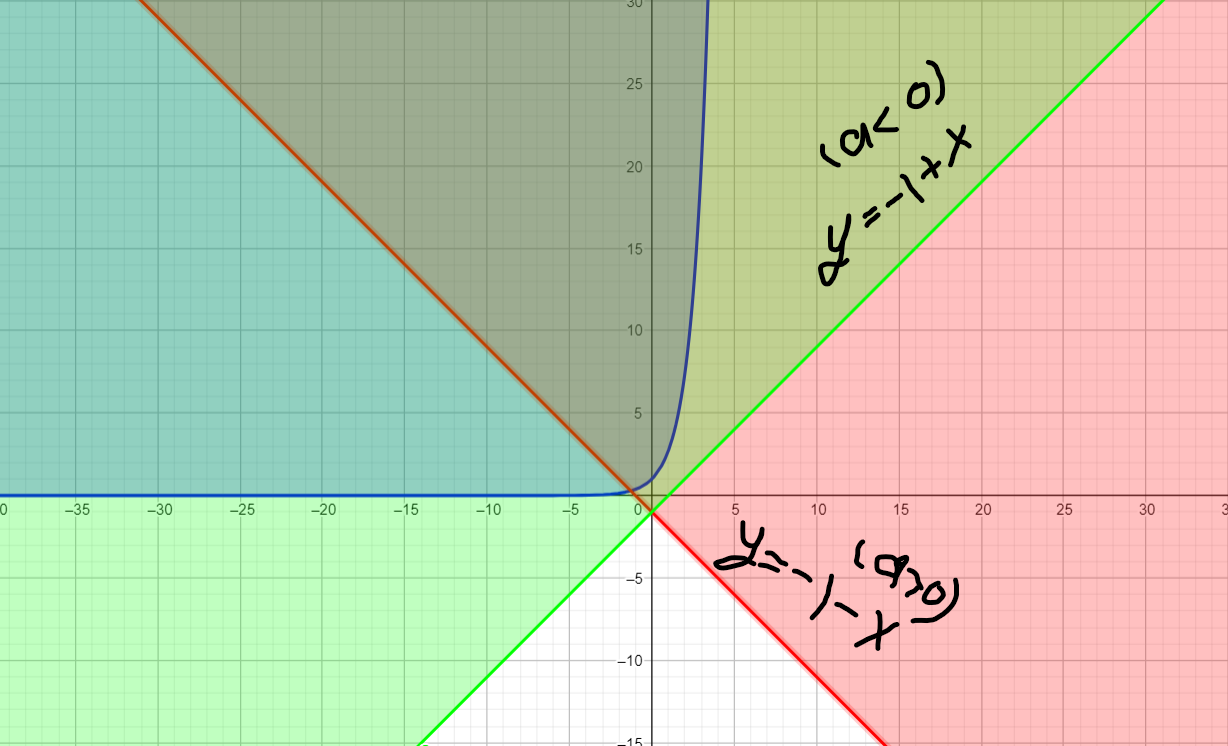
\includegraphics[width=\textwidth]{pictures/task_05_04.png}}
    \caption{$c = 1$}
\end{figure}

    

    \item $c = 0$, $\not \exists a, b$ such that all values of $at + b\geq 0$ lie above $p \geq e^t$. It's vertical line.

    \item $c = -1$, All points $p \geq e^t$ must lie above $p \leq at + b$, but $\not \exists a,b$.
\end{enumerate}


\begin{figure}
  \centering
    \fbox{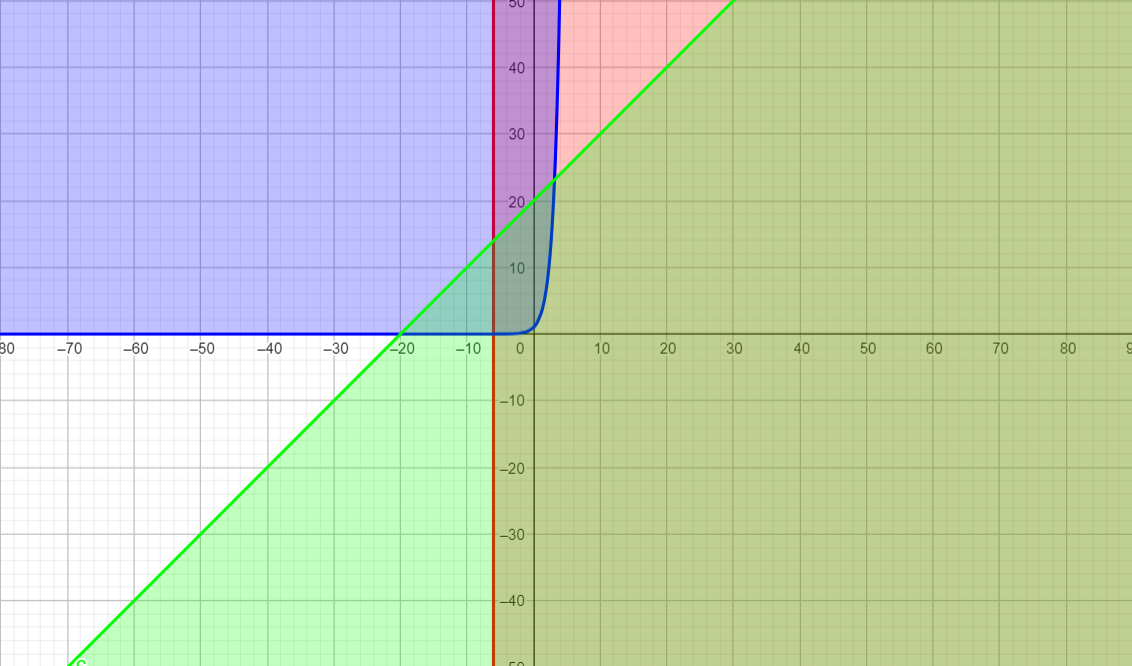
\includegraphics[width=\textwidth]{pictures/task_05_05.png}}
    \caption{$c = 0$ and $c < 0$}
\end{figure}

All others solutions could get by mupltipluyng c on some positive constant.

\underline{\textbf{Answer:}}

\begin{equation*}
K^{*} = \left\{ (c \cdot a, c \cdot b, c) \text{ | } c\geq 0\text{, if } a = 0 \text{ and } b \geq 0 \text{, or } a < 0 \text{ and } b \geq a(1-\ln(-a)) \right\}
\end{equation*}